\documentclass[a4paper]{article}

\usepackage[utf8]{inputenc}
\usepackage[T1]{fontenc}
\usepackage[italian]{babel}

\usepackage[margin=4.5cm, top=1.5cm, bottom=2.5cm]{geometry}

\usepackage{siunitx}
\usepackage{amsmath}
\usepackage{amssymb}
\usepackage[hidelinks]{hyperref}
\usepackage{graphicx}
\usepackage[font={sf}]{caption}

\setlength{\marginparwidth}{95pt}
\let\oldmarginpar\marginpar
\renewcommand\marginpar[1]{\oldmarginpar{\scriptsize\sffamily #1}}

\sisetup{%
separate-uncertainty=true,
multi-part-units=single,
exponent-product=\cdot}

\frenchspacing

\begin{document}

\subsection{Effetto del materiale sulla misura}

Abbiamo testato quanto la presenza di lastre di piombo potesse influire sulla rivelazione dei raggi cosmici. Abbiamo a disposizione il seguente materiale:
\begin{itemize}

\item 3 lastre rigide di piombo\\
spessore=\SI{4\pm1}{mm}\\
L1=\SI{39.9\pm0.1}{ cm}\\
L2=\SI{40.0\pm0.1}{cm}

\item 1 lastra di alluminio con le stesse dimensioni delle 3 precedenti

\item 10 lastre flessibili di piombo\\
spessore=\SI{2\pm1}{ mm}\\
L1=\SI{47.5\pm0.1}{ cm}\\
L2=\SI{45.0\pm0.1}{ cm}

\end{itemize}

\subsubsection{Conteggi}

Abbiamo posizionato le lastre rigide tra il PM3 ed il PM4 per vedere se esse riuscivano a fermare parte dei muoni. Per fare questa misura abbiamo confrontato le coincidenze  PM5 \& PM4 e PM5 \& PM4 \& PM3, però non possiamo confrontarle così come sono a causa dell'accettanza geometrica: anche in assenza delle lastre le coincidenze a tre sono diverse da quelle a due. Allora correggiamo le coincidenze a due con un Monte Carlo che tiene in considerazione le efficienze dei tre rivelatori. Il fattore di correzione ottenuto è il rapporto tra le accettanze delle due configurazioni  $\delta=mc(\text{PM5 \& PM4 \&PM3})/mc(\text{PM5 \& PM4})=65.71\pm0.02\%$, dove $mc$ indica il risultato del Monte Carlo per la configurazione in questione. Siano $C2$ il numero di coincidenze a due e $C3$ il numero di quelle a tre, per capire quanto sia significativo l'effetto delle lastre sulle nostre misure confrontiamo le quantità $C2'=C2 \cdot \delta$ e $C3$ in funzione del numero di lastre inserite%
\footnote{Nel grafico di \autoref{cfr} non è presente il caso di 3 lastre perché, avendone una di alluminio, abbiamo deciso di metterla insieme alla terza lastra di piombo.}. %
Dal confronto, presente in \autoref{cfr}, non si evince nessuna differenza tra i conteggi a meno di una separazione di $3\sigma$ nell'ultimo caso che, come descritto nella sezione successiva, rappresenta solo una fluttuazione.
\marginpar{scrivere il tempo di misura || $3\sigma$ l'ho detto ad occhio || giustificazione nella sezione successiva}

\begin{figure}[h]
\centering
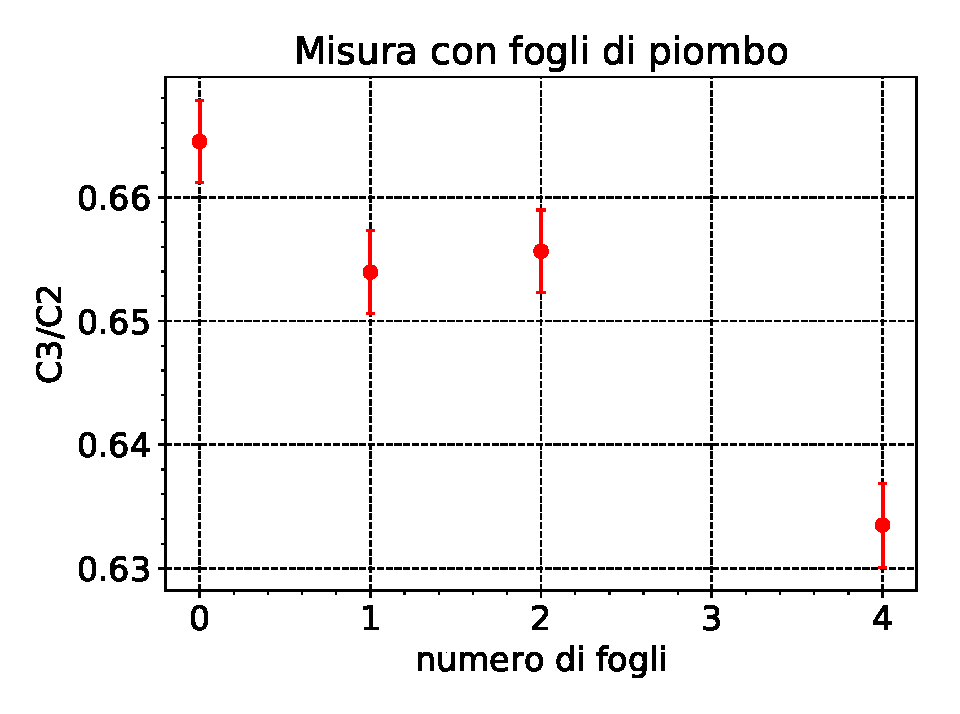
\includegraphics[width=8 cm]{confronto}
\caption{Confronto tra le coincidenze a due corrette e quelle a tre in funzione del numero di lastre inserite sul PM3.}
\label{cfr}
\end{figure}

\subsubsection{Energia}

\end{document}